\sloppy
\documentclass[14pt,a4paper,twoside]{extarticle}	% Размер основного шрифта и формата листа
\usepackage{xltxtra}						% Используется для вывода логотипа XeLaTeX
\usepackage{xunicode}						% Кодировка документа
\usepackage{polyglossia}					% Загружает пакет многоязыковой верстки
\newfontfamily\russianfont{Book Antiqua}
%\setmainfont{Liberation Serif}						% Основной шрифт текста
\setmainfont{Book Antiqua}
\setdefaultlanguage{russian}				% Основной язык текста
\setotherlanguage{english}					% Дополнительный язык текста
\linespread{1}							% Межстрочный интервал выбран полуторным
\usepackage[left=2.5cm,
right=1.5cm,vmargin=2.5cm]{geometry} % Отступы по краям листа
\bibliographystyle{ugost2008}

\usepackage{xcolor}
\usepackage{hyperref}
% Цвета для гиперссылок
\definecolor{linkcolor}{HTML}{359B08} % цвет ссылок
\definecolor{urlcolor}{HTML}{799B03} % цвет гиперссылок
\hypersetup{pdfstartview=FitH,  linkcolor=linkcolor,urlcolor=urlcolor, colorlinks=true}

%---------------------------%
%---- Пакеты расширений ----%
%---------------------------%
\usepackage{xcolor}
\usepackage{hyperref}
% Цвета для гиперссылок
\definecolor{linkcolor}{HTML}{359B08} % цвет ссылок
\definecolor{urlcolor}{HTML}{799B03} % цвет гиперссылок
\hypersetup{pdfstartview=FitH,  linkcolor=linkcolor,urlcolor=urlcolor, colorlinks=true}


\usepackage{verbatim,indentfirst}
\usepackage{cite,enumerate,float}
\usepackage{amsmath,amssymb,amsthm,amsfonts}

%---------------------------%
%--- Вставка иллюстраций ---%
%---------------------------%
\usepackage{graphicx}
\usepackage{subfigure}
%\graphicspath{{Images/}}
\usepackage{fontspec}

\begin{document}
%	\pagestyle{empty} %  выключаенм нумерацию
%\setcounter{page}{3}% Нумерация начинается с третьей страницы
%\renewcommand{\contentsname}{\center{Содержание}}
%\tableofcontents
	
\newpage
\begin{center}
	%\addcontentsline{toc}{section}{Сила Кориолиса}
	\subsection*{Сбрасывание цепочки с вращающегося диска}
\end{center}
		
\begin{figure}[H] 	
	\centering 	
		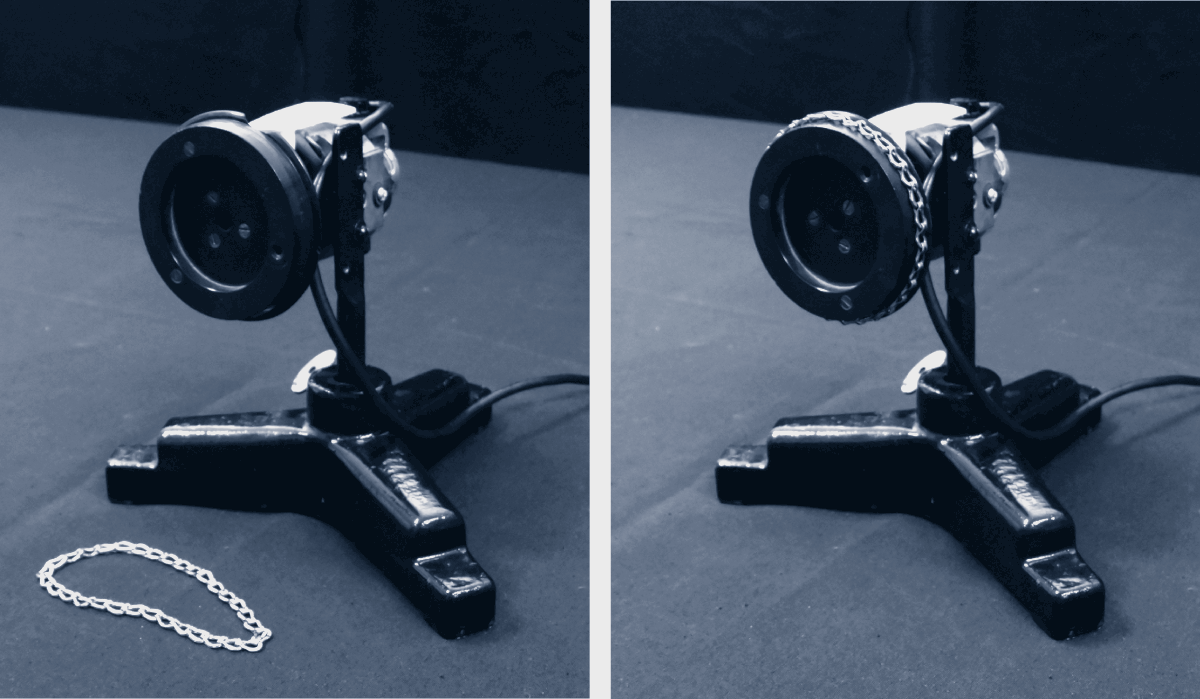
\includegraphics[width=0.9\linewidth]{chain-1.png}
		\caption{Демонстрация устойчивости движения вращающейся цепочки под действием центробежных сил инерции}
		\label{chain-1}
	\end{figure}
		
		\subsection*{\underline{Оборудование:}}
		
		\begin{enumerate}
			\item Диск с цепочкой
			\item Электродвигатель универсальный
			\item Лабораторный трансформатор
			\item Штатив универсальный
			\item Металлическая пластинка
		\end{enumerate}
		
		\subsection*{\underline{Основные определения:}}
		
		НАЙТИ
		
		\subsection*{\underline{Краткое описание:}}
				
		Специальный шкив с надетой на него замкнутой в кольцо цепочкой закрепляют на валу универсального электродвигателя.
		Подавая напряжение от трансформатора вал двигателя раскручивается и при большом числе оборотов жесткой плоской пластинкой цепочку сбрасывают со шкива.
		Цепочка начинает катиться по столу как жесткое упругое кольцо.

	\begin{figure}[H] 	
	\centering 	
	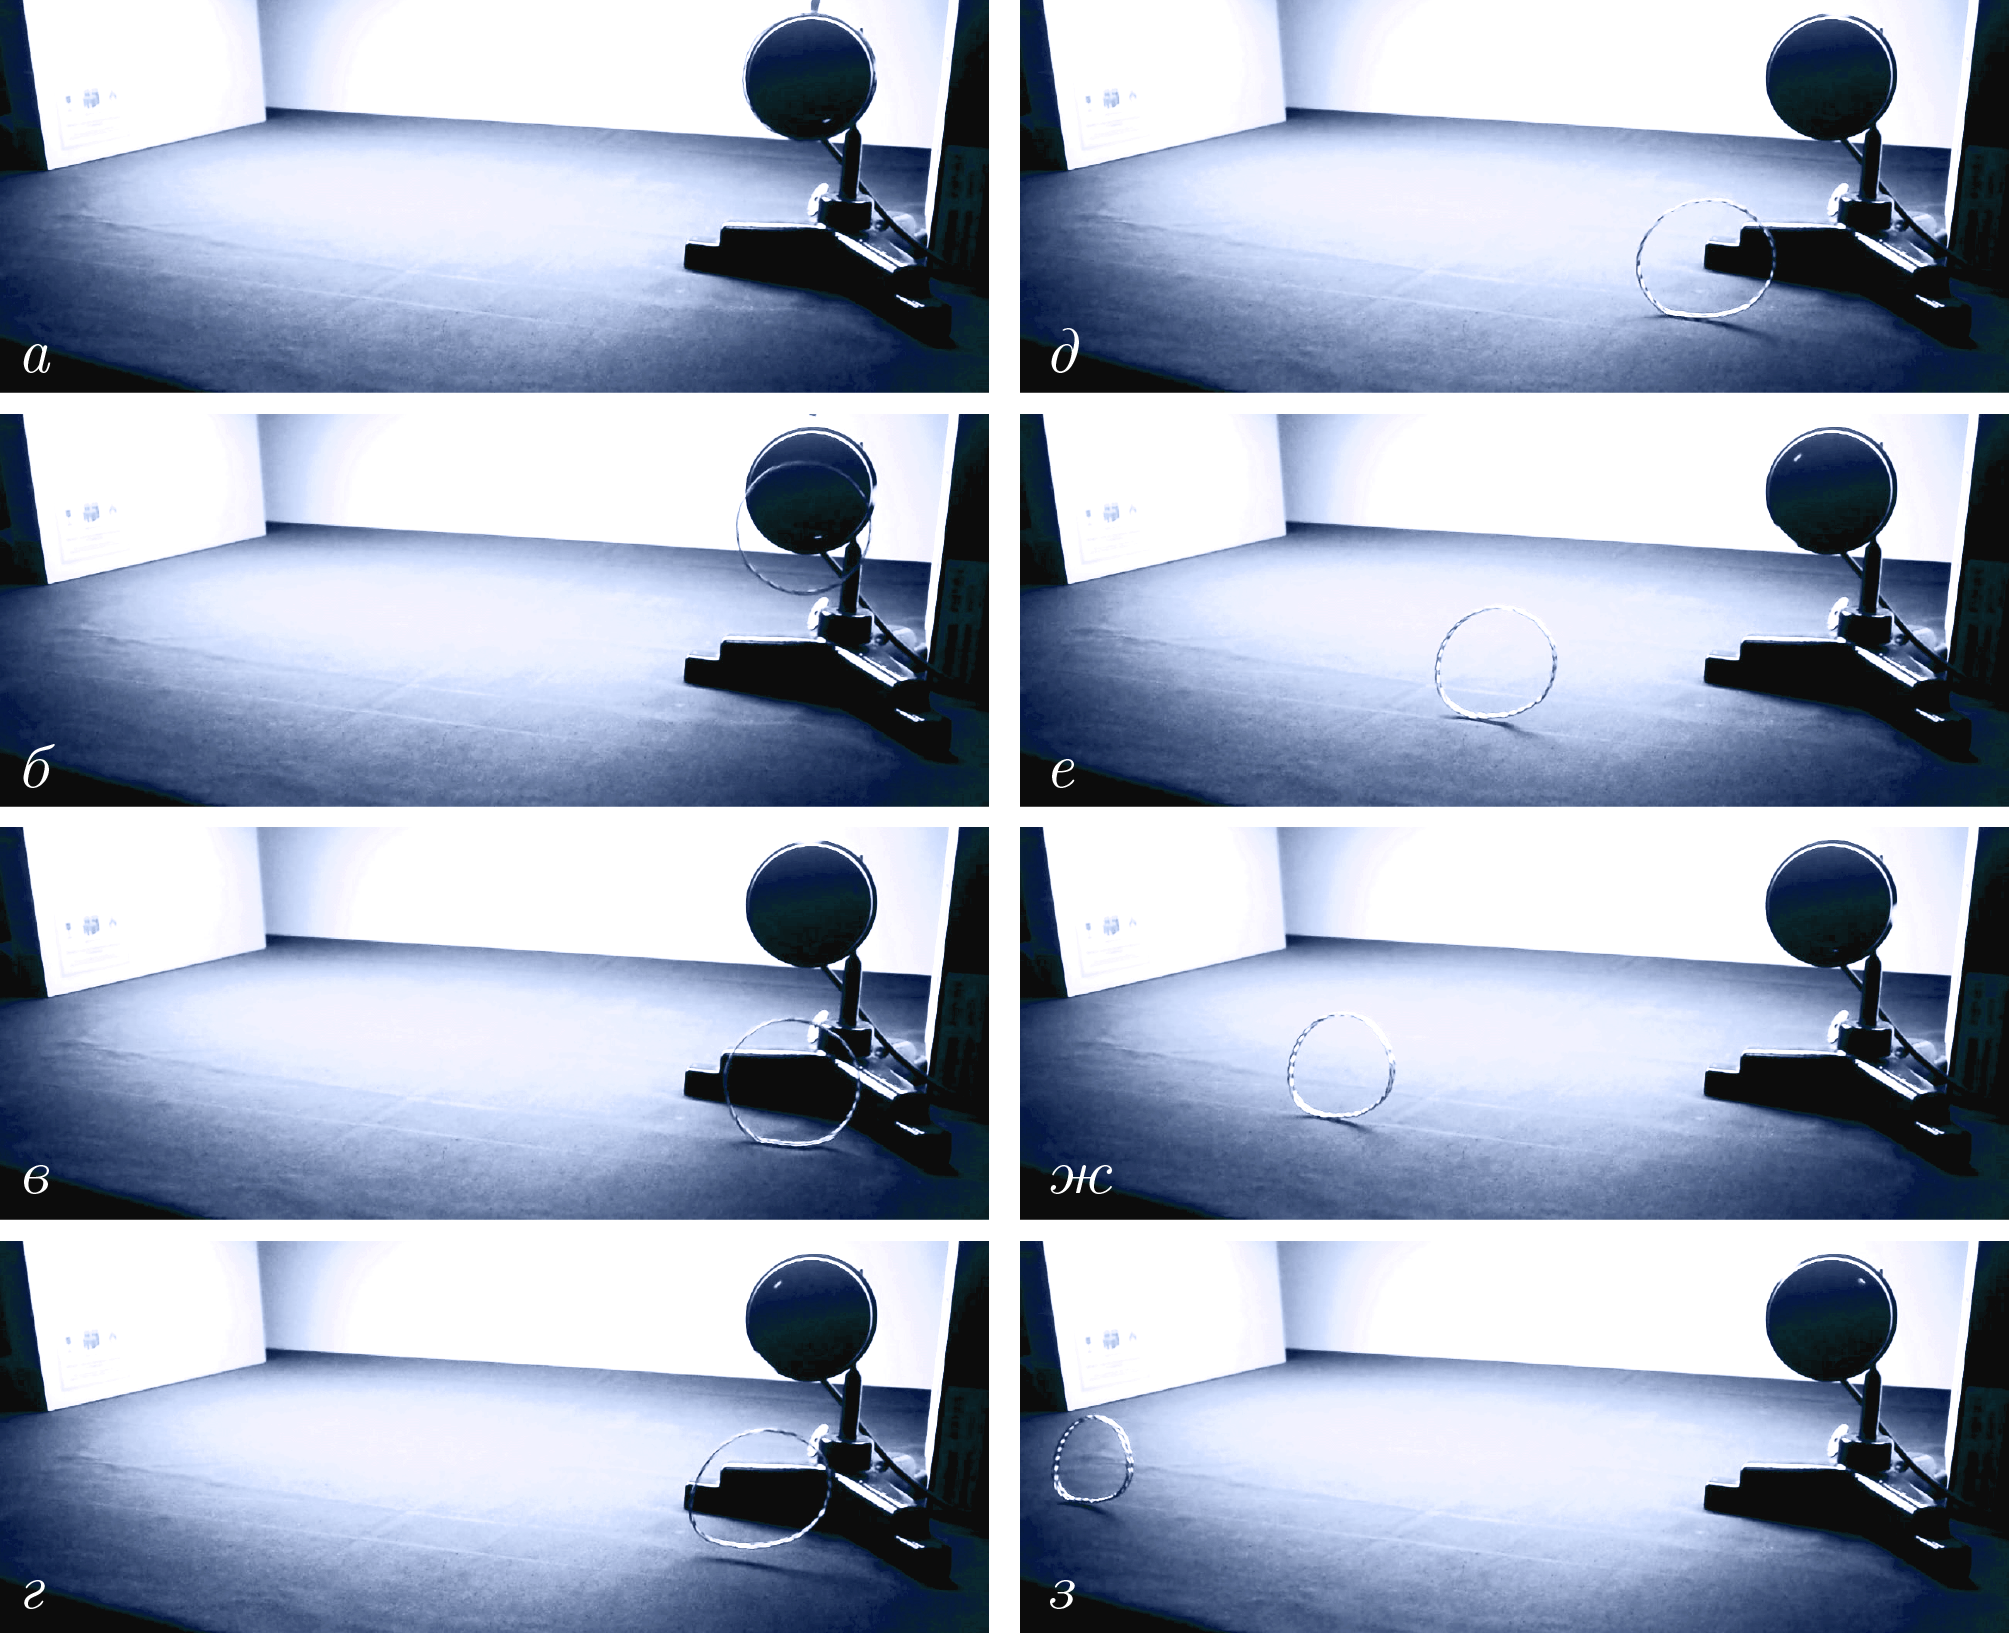
\includegraphics[width=0.9\linewidth]{chain-2.png}
	\caption{Сбрасывание цепочки с вращающегося диска. Возникновение силы инерции приводит к тому, что цепочка движется вдоль поверхности стола как упругое кольцо, продолжая вращаться}
	\label{chain-2}
\end{figure}
		
	\subsection*{\underline{Теория:}}
		
Эффект устойчивого вращения деформируемой цепочки обусловлен возникновением силы, действующей на каждое из звеньев цепочки, которая сообщает ему нормальное ускорение.
В начале движения каждое звено цепочки движется по инерции прямолинейно, пока цепочка не натянется.
Причем каждое звено удерживается на окружности силами упругости двух соседних звеньев (рис.\ref{chain-3}).
		
\begin{figure}[H] 	
	\centering 	
	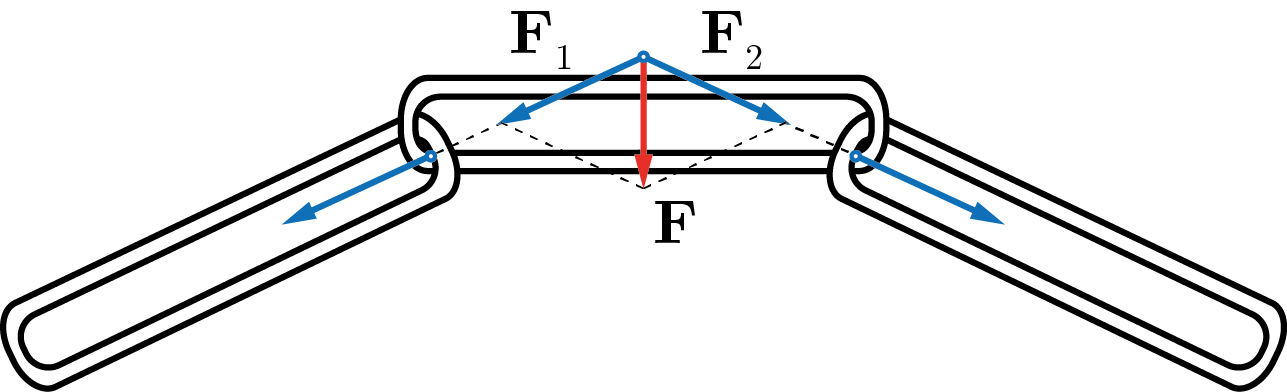
\includegraphics[width=0.75\linewidth]{chain-3.png}
	\caption{Схема распределения сил в звеньях натянутой в результате вращения цепочки}
	\label{chain-3}
\end{figure}
	
Равнодействующая этих сил и есть та сила, которая сообщает звену нормальное ускорение.
		
		
		
	\end{document}